% GNUPLOT: LaTeX picture with Postscript
\begingroup
  % Encoding inside the plot.  In the header of your document, this encoding
  % should to defined, e.g., by using
  % \usepackage[latin1,<other encodings>]{inputenc}
  \inputencoding{latin1}%
  \makeatletter
  \providecommand\color[2][]{%
    \GenericError{(gnuplot) \space\space\space\@spaces}{%
      Package color not loaded in conjunction with
      terminal option `colourtext'%
    }{See the gnuplot documentation for explanation.%
    }{Either use 'blacktext' in gnuplot or load the package
      color.sty in LaTeX.}%
    \renewcommand\color[2][]{}%
  }%
  \providecommand\includegraphics[2][]{%
    \GenericError{(gnuplot) \space\space\space\@spaces}{%
      Package graphicx or graphics not loaded%
    }{See the gnuplot documentation for explanation.%
    }{The gnuplot epslatex terminal needs graphicx.sty or graphics.sty.}%
    \renewcommand\includegraphics[2][]{}%
  }%
  \providecommand\rotatebox[2]{#2}%
  \@ifundefined{ifGPcolor}{%
    \newif\ifGPcolor
    \GPcolortrue
  }{}%
  \@ifundefined{ifGPblacktext}{%
    \newif\ifGPblacktext
    \GPblacktexttrue
  }{}%
  % define a \g@addto@macro without @ in the name:
  \let\gplgaddtomacro\g@addto@macro
  % define empty templates for all commands taking text:
  \gdef\gplbacktext{}%
  \gdef\gplfronttext{}%
  \makeatother
  \ifGPblacktext
    % no textcolor at all
    \def\colorrgb#1{}%
    \def\colorgray#1{}%
  \else
    % gray or color?
    \ifGPcolor
      \def\colorrgb#1{\color[rgb]{#1}}%
      \def\colorgray#1{\color[gray]{#1}}%
      \expandafter\def\csname LTw\endcsname{\color{white}}%
      \expandafter\def\csname LTb\endcsname{\color{black}}%
      \expandafter\def\csname LTa\endcsname{\color{black}}%
      \expandafter\def\csname LT0\endcsname{\color[rgb]{1,0,0}}%
      \expandafter\def\csname LT1\endcsname{\color[rgb]{0,1,0}}%
      \expandafter\def\csname LT2\endcsname{\color[rgb]{0,0,1}}%
      \expandafter\def\csname LT3\endcsname{\color[rgb]{1,0,1}}%
      \expandafter\def\csname LT4\endcsname{\color[rgb]{0,1,1}}%
      \expandafter\def\csname LT5\endcsname{\color[rgb]{1,1,0}}%
      \expandafter\def\csname LT6\endcsname{\color[rgb]{0,0,0}}%
      \expandafter\def\csname LT7\endcsname{\color[rgb]{1,0.3,0}}%
      \expandafter\def\csname LT8\endcsname{\color[rgb]{0.5,0.5,0.5}}%
    \else
      % gray
      \def\colorrgb#1{\color{black}}%
      \def\colorgray#1{\color[gray]{#1}}%
      \expandafter\def\csname LTw\endcsname{\color{white}}%
      \expandafter\def\csname LTb\endcsname{\color{black}}%
      \expandafter\def\csname LTa\endcsname{\color{black}}%
      \expandafter\def\csname LT0\endcsname{\color{black}}%
      \expandafter\def\csname LT1\endcsname{\color{black}}%
      \expandafter\def\csname LT2\endcsname{\color{black}}%
      \expandafter\def\csname LT3\endcsname{\color{black}}%
      \expandafter\def\csname LT4\endcsname{\color{black}}%
      \expandafter\def\csname LT5\endcsname{\color{black}}%
      \expandafter\def\csname LT6\endcsname{\color{black}}%
      \expandafter\def\csname LT7\endcsname{\color{black}}%
      \expandafter\def\csname LT8\endcsname{\color{black}}%
    \fi
  \fi
    \setlength{\unitlength}{0.0500bp}%
    \ifx\gptboxheight\undefined%
      \newlength{\gptboxheight}%
      \newlength{\gptboxwidth}%
      \newsavebox{\gptboxtext}%
    \fi%
    \setlength{\fboxrule}{0.5pt}%
    \setlength{\fboxsep}{1pt}%
\begin{picture}(5760.00,3876.00)%
    \gplgaddtomacro\gplbacktext{%
      \csname LTb\endcsname%
      \put(330,777){\makebox(0,0){\fontsize{6}{6}\selectfont{5}}}%
      \put(330,1454){\makebox(0,0){\fontsize{6}{6}\selectfont{10}}}%
      \put(330,2131){\makebox(0,0){\fontsize{6}{6}\selectfont{15}}}%
      \put(330,2809){\makebox(0,0){\fontsize{6}{6}\selectfont{20}}}%
      \put(567,330){\rotatebox{45}{\makebox(0,0)[l]{\strut{}\fontsize{5}{5}\selectfont{8,1}}}}%
      \put(723,330){\rotatebox{45}{\makebox(0,0)[l]{\strut{}\fontsize{5}{5}\selectfont{7,2}}}}%
      \put(880,330){\rotatebox{45}{\makebox(0,0)[l]{\strut{}\fontsize{5}{5}\selectfont{6,3}}}}%
      \put(1036,330){\rotatebox{45}{\makebox(0,0)[l]{\strut{}\fontsize{5}{5}\selectfont{5,4}}}}%
      \put(1193,330){\rotatebox{45}{\makebox(0,0)[l]{\strut{}\fontsize{5}{5}\selectfont{4,5}}}}%
      \put(1349,330){\rotatebox{45}{\makebox(0,0)[l]{\strut{}\fontsize{5}{5}\selectfont{3,6}}}}%
      \put(1506,330){\rotatebox{45}{\makebox(0,0)[l]{\strut{}\fontsize{5}{5}\selectfont{2,7}}}}%
      \put(1662,330){\rotatebox{45}{\makebox(0,0)[l]{\strut{}\fontsize{5}{5}\selectfont{1,8}}}}%
      \put(1819,330){\rotatebox{45}{\makebox(0,0)[l]{\strut{}\fontsize{5}{5}\selectfont{8,0}}}}%
      \put(1975,330){\rotatebox{45}{\makebox(0,0)[l]{\strut{}\fontsize{5}{5}\selectfont{7,1}}}}%
      \put(2132,330){\rotatebox{45}{\makebox(0,0)[l]{\strut{}\fontsize{5}{5}\selectfont{6,2}}}}%
      \put(2288,330){\rotatebox{45}{\makebox(0,0)[l]{\strut{}\fontsize{5}{5}\selectfont{5,3}}}}%
      \put(2445,330){\rotatebox{45}{\makebox(0,0)[l]{\strut{}\fontsize{5}{5}\selectfont{4,4}}}}%
      \put(2601,330){\rotatebox{45}{\makebox(0,0)[l]{\strut{}\fontsize{5}{5}\selectfont{3,5}}}}%
      \put(2758,330){\rotatebox{45}{\makebox(0,0)[l]{\strut{}\fontsize{5}{5}\selectfont{2,6}}}}%
      \put(2914,330){\rotatebox{45}{\makebox(0,0)[l]{\strut{}\fontsize{5}{5}\selectfont{1,7}}}}%
      \put(3071,330){\rotatebox{45}{\makebox(0,0)[l]{\strut{}\fontsize{5}{5}\selectfont{0,8}}}}%
      \put(3227,330){\rotatebox{45}{\makebox(0,0)[l]{\strut{}\fontsize{5}{5}\selectfont{7,0}}}}%
      \put(3384,330){\rotatebox{45}{\makebox(0,0)[l]{\strut{}\fontsize{5}{5}\selectfont{6,1}}}}%
      \put(3540,330){\rotatebox{45}{\makebox(0,0)[l]{\strut{}\fontsize{5}{5}\selectfont{5,2}}}}%
      \put(3697,330){\rotatebox{45}{\makebox(0,0)[l]{\strut{}\fontsize{5}{5}\selectfont{4,3}}}}%
      \put(3853,330){\rotatebox{45}{\makebox(0,0)[l]{\strut{}\fontsize{5}{5}\selectfont{3,4}}}}%
      \put(4010,330){\rotatebox{45}{\makebox(0,0)[l]{\strut{}\fontsize{5}{5}\selectfont{2,5}}}}%
      \put(4166,330){\rotatebox{45}{\makebox(0,0)[l]{\strut{}\fontsize{5}{5}\selectfont{1,6}}}}%
      \put(4323,330){\rotatebox{45}{\makebox(0,0)[l]{\strut{}\fontsize{5}{5}\selectfont{0,7}}}}%
      \put(4479,330){\rotatebox{45}{\makebox(0,0)[l]{\strut{}\fontsize{5}{5}\selectfont{6,0}}}}%
      \put(4636,330){\rotatebox{45}{\makebox(0,0)[l]{\strut{}\fontsize{5}{5}\selectfont{5,1}}}}%
      \put(4792,330){\rotatebox{45}{\makebox(0,0)[l]{\strut{}\fontsize{5}{5}\selectfont{4,2}}}}%
      \put(4949,330){\rotatebox{45}{\makebox(0,0)[l]{\strut{}\fontsize{5}{5}\selectfont{3,3}}}}%
      \put(5105,330){\rotatebox{45}{\makebox(0,0)[l]{\strut{}\fontsize{5}{5}\selectfont{2,4}}}}%
      \put(5262,330){\rotatebox{45}{\makebox(0,0)[l]{\strut{}\fontsize{5}{5}\selectfont{1,5}}}}%
      \put(5418,330){\rotatebox{45}{\makebox(0,0)[l]{\strut{}\fontsize{5}{5}\selectfont{0,6}}}}%
    }%
    \gplgaddtomacro\gplfronttext{%
      \csname LTb\endcsname%
      \put(22,1860){\rotatebox{-270}{\makebox(0,0){\strut{}\footnotesize Costo global $T$}}}%
      \put(3044,88){\makebox(0,0){\strut{}\footnotesize Objetos en malla (cubos, prismas)}}%
      \put(3044,3545){\makebox(0,0){\strut{}\large Resultados en mallas de $\mathsf{3\times 3}$}}%
      \csname LTb\endcsname%
      \put(5036,3069){\makebox(0,0)[r]{\strut{}\fontsize{6}{6}\selectfont{B\'usqueda exhaustiva}}}%
      \csname LTb\endcsname%
      \put(5036,2904){\makebox(0,0)[r]{\strut{}\fontsize{6}{6}\selectfont{B\'usqueda por RS}}}%
    }%
    \gplbacktext
    \put(0,0){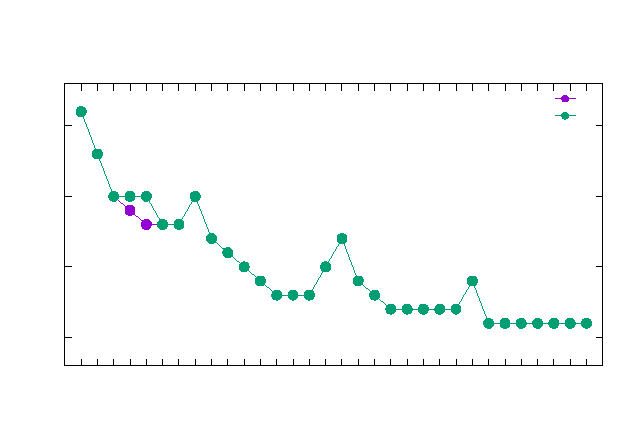
\includegraphics{comparacionAlgoritmos3x3}}%
    \gplfronttext
  \end{picture}%
\endgroup
